\documentclass[11pt]{article}
\usepackage[UTF8]{ctex}
\usepackage[a4paper]{geometry}
\geometry{left=2.0cm,right=2.0cm,top=2.5cm,bottom=2.5cm}

\usepackage{caption}
\usepackage{paralist}
\usepackage{enumitem}
\setenumerate[1]{itemsep=0pt,partopsep=0pt,parsep=0pt,topsep=0pt}
\setitemize[1]{itemsep=0pt,partopsep=0pt,parsep=0pt,topsep=0pt}
\usepackage{comment}
\usepackage{booktabs}
\usepackage{float}
\usepackage{diagbox}
\usepackage{amsmath,amsfonts,graphicx,amssymb,bm,amsthm}
\usepackage{algorithm,algorithmicx}
% \usepackage[ruled, linesnumbered]{algorithm2e}
% \usepackage[linesnumbered]{algorithm2e}
\usepackage[noend]{algpseudocode}
\usepackage{fancyhdr}
\usepackage{tikz}
\usepackage{tikz-qtree}
\usepackage{graphicx}
\usetikzlibrary{arrows,automata, positioning}
\usepackage{hyperref}
\usepackage{extarrows}
% 这是一些字体选项
\usepackage{helvet}
% \usepackage{mathpazo}
\usepackage{fontspec}
% \setmainfont{Times New Roman}
% \setmainfont{Comic Sans MS} % 比较fancy的字体
% \setmainfont{Avenir}
% \setmainfont{Palatino}

\RequirePackage{algorithm}

\makeatletter
\newenvironment{breakablealgorithm}
  {% \begin{breakablealgorithm}
    \begin{center}
      \refstepcounter{algorithm}% New algorithm
      \hrule height.8pt depth0pt \kern2pt% \@fs@pre for \@fs@ruled
      \parskip 0pt
      \renewcommand{\caption}[2][\relax]{% Make a new \caption
        {\raggedright\textbf{\fname@algorithm~\thealgorithm} ##2\par}%
        \ifx\relax##1\relax % #1 is \relax
          \addcontentsline{loa}{algorithm}{\protect\numberline{\thealgorithm}##2}%
        \else % #1 is not \relax
          \addcontentsline{loa}{algorithm}{\protect\numberline{\thealgorithm}##1}%
        \fi
        \kern2pt\hrule\kern2pt
     }
  }
  {% \end{breakablealgorithm}
     \kern2pt\hrule\relax% \@fs@post for \@fs@ruled
   \end{center}
  }
\makeatother

% set for automata
% \tikzset{
%         % ->,  % makes the edges directed
%         % >=stealth, % makes the arrow heads bold
%         node distance=5cm, % specifies the minimum distance between two nodes. Change if n
%         every state/.style={thick, fill=gray!10}, % sets the properties for each ’state’ n
%         initial text=$start$, % sets the text that appears on the start arrow
%         }

\setlength{\headheight}{14pt}
\setlength{\parindent}{0 in}
\setlength{\parskip}{0.5 em}


\newtheorem{theorem}{Theorem}
\newtheorem{lemma}[theorem]{Lemma}
\newtheorem{proposition}[theorem]{Proposition}
\newtheorem{claim}[theorem]{Claim}
\newtheorem{corollary}[theorem]{Corollary}
\newtheorem{definition}[theorem]{Definition}
\newtheorem*{definition*}{Definition}
\newcommand{\mP}{\mathbf{P}}
\newcommand{\NP}{\mathbf{NP}}
\newcommand{\NPC}{\mathbf{NP}\text{-complete}}
\newcommand{\coNP}{\mathbf{coNP}}
\newcommand{\PSPACE}{\mathbf{PSPACE}}
\newcommand{\PSPACEC}{\mathbf{PSPACE}\text{-complete}}
\newcommand{\EXP}{\mathbf{EXP}}
\newcommand{\NEXP}{\mathbf{NEXP}}
\newcommand{\BPP}{\mathbf{BPP}}
\newcommand{\RP}{\mathbf{RP}}
\newcommand{\ZPP}{\mathbf{ZPP}}
\newcommand{\LL}{\mathbf{L}}
\newcommand{\NL}{ \mathbf{NL}}
\newcommand{\NLC}{\mathbf{NL}\text{-complete}}
\newcommand{\PP}{\mathbb{P}}
\newcommand{\NC}{\mathbf{NC}}
\newcommand{\PH}{\mathbf{PH}}
\newcommand{\1}{\mathbf{1}}


\newenvironment{problem}[2][Problem]{\begin{trivlist}
\item[\hskip \labelsep{\bfseries#1}\hskip\labelsep{\bfseries#2.}]}{\hfill$\blacktriangleleft$\end{trivlist}}
\newenvironment{answer}[1][Answer]{\begin{trivlist}
\item[\hskip \labelsep{\bfseries\itshape#1.}\hskip \labelsep]}{\hfill$\lhd$\end{trivlist}}

\newcommand\E{\mathbb{E}}
\newcommand\per{\mathrm{per}}
\renewcommand{\algorithmicrequire}{\textbf{Input:}}
\renewcommand{\algorithmicensure}{\textbf{Output:}}
\algrenewcommand{\algorithmiccomment}[1]{\hfill $//$ #1}
% chktex-file 44
% \renewcommand{\familydefault}{\sfdefault}

\title{Homework \#3}
\usetikzlibrary{positioning}

\begin{document}
\captionsetup[figure]{labelfont={bf},name={Fig.},labelsep=period}
\kaishu

\pagestyle{fancy}
\lhead{\CJKfamily{zhkai} Peking University}
\chead{}
\rhead{\CJKfamily{zhkai} Introduction to Theory of Computation, 2024 Spring}

\begin{center}
    {\LARGE \bf Homework 5}\\
    {Name: 方嘉聪\ \  ID: 2200017849}            % Write down your name and ID here.
\end{center}

\begin{problem}{1(16 points)}
    Prove that every function $f: \{0,1\}^n \rightarrow \{0,1\}$ can be computed by a circuit of size less than $10\cdot 2^n$.
\end{problem}
\begin{answer}
    不妨设一个布尔函数为$f(x_1,x_2,\cdots,x_n)$, 考虑如下的分解:
    \begin{align}
        \label{decompose}
        f(x_1, x_2,\cdots,x_n) = (x_1 \land f(1, x_2, \cdots, x_n)) \lor (\neg x_1 \land f(0, x_2, \cdots, x_n))
    \end{align}
    具体的, 分解\eqref{decompose}对应的电路如下:
    \begin{center}
        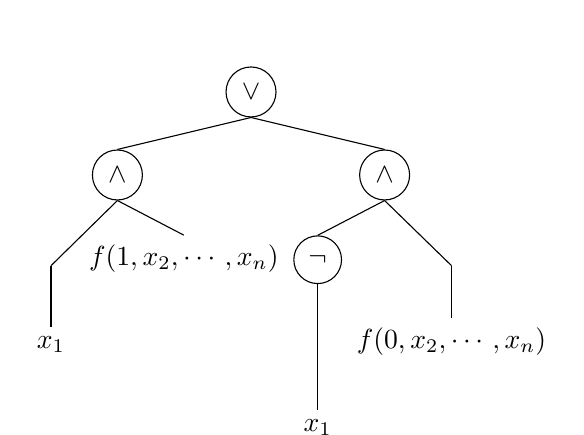
\begin{tikzpicture}
            \Tree 
            [.\node[draw,circle]{$\lor$};
                [.\node[draw,circle]{$\land$}; [$x_1$ ] [.$f(1,x_2,\cdots,x_n)$ ]]
                [.\node[draw,circle]{$\land$}; [.\node[draw,circle]{$\neg$}; [$x_1$ ]] [$f(0,x_2,\cdots,x_n)$ ]]
            ]
        \end{tikzpicture}
    \end{center}
    迭代的重复上述分解. 设$T(n)$为计算$f(x_1, x_2,\cdots,x_n)$的电路大小, 则有(注意到$T(1) \le 1$):
    \begin{align*}
        T(n) \leq 2T(n-1) + 4 \implies T(n) \le 2^{n-1}(T(1) + 4) - 4 < 10 \cdot 2^n
    \end{align*}
    证毕. 
\end{answer}
\begin{problem}{2(21 points)}
    Improve this bound to show that every function $f: \{0,1\}^n \rightarrow \{0,1\}$ can be computed by a circuit of size less than $1000\cdot 2^n/n$.
\end{problem}
\begin{answer}
    大致思路: 考虑第一题的分解\eqref{decompose}, 运行$n-k$步之后, 不再继续分解下去, 而是选择去计算\textbf{所有}的布尔函数在最后$k$位上的结果, 这样可以实现电路的复用, 从而得到一个电路大小更优的上界. \textcolor{red}{当$n$比较小时, 会有$1000\cdot 2^n/n < 10\cdot 2^n$, 直接使用第一题的分解即可, 下面考虑$n$较大的情况:  }
    
    具体的, 设函数$g_k:\{0,1\}^k \rightarrow \{0,1\}^{2^{2^k}}$表示输入长度为$k$时所有可能的布尔函数的输出, 即:
    \begin{align*}
        g_k(x_1, x_2, \cdots, x_k) = (f_1(x_1, x_2, \cdots, x_k), f_2(x_1, x_2, \cdots, x_k), \cdots, f_{2^{2^k}}(x_1, x_2, \cdots, x_k))
    \end{align*}
    其中$f_i$表示第$i$个布尔函数. 由第一题知计算$g_k$所需电路大小的上界为$10\cdot 2^k\cdot 2^{2^k}$. 

    那么对于$f(x_1, x_2, \cdots, x_n)$, 我们先预处理得到$g_k$对应的电路, 而后运行第一题的分解方式$n-k$轮, 余下的$k$轮直接计算$g_k$的输出. 于是总的电路大小上界$\mathcal{C}(f)$为:
    \begin{align*}
        \mathcal{C}(f) &\le 10\cdot 2^{k}\cdot 2^{2^{k}} + 4 (2^0 + 2^1 + \cdots + 2^{n-k-1}) \\
         &= 10\cdot 2^{k}\cdot 2^{2^{k}} + 4(2^{n-k} - 1) \\
         [\text{let } k = \log_2(n)-1] &< 10\cdot 2^{\log_2(n) - 1 + n/2} + 4\cdot 2^{n + 1-\log_2(n)} \\ 
         &= \left(\frac{5n^2}{2^{n/2}} + 8\right)\frac{2^n}{n} < 1000\cdot \frac{2^n}{n}
    \end{align*}
    设$t(n) = 5n^2/2^{n/2}$, 那么$t'(n) = (4n - \ln 2\cdot n^2)/2^{n/2+1}$, 故$\max t(n) < t(4/\ln 2) < 1000$, 故上述最后一个不等号成立, 证毕.
    
    注: 1000看起来是一个比较松的常数, 这里$k$也可以取其他的值. 如果考虑渐进复杂度, 可以证明
    \begin{align*}
        \mathcal{C}(g_k) \le 2^{2^k}(1 + o(1)) \implies  \mathcal{C}(f) = (1 + o(1))\frac{2^n}{n}.
    \end{align*}
    % 这里不再展开\footnote{参考了\url{https://nitinsau.github.io/teaching/BFC19-mpii/lecture2.pdf}}. 
\end{answer}

\begin{problem}{3(21 points)}
    Show that for every $k > 0$ that $\PH$ contains languages whose circuit complexity is $\Omega(n^k)$.
\end{problem}
\begin{answer}
    我们先来证明如下的引理:
    \begin{lemma}
        $\forall n,k\in\mathbf{N}^+$, 存在一个大小为$2\cdot n^{2k+2}$的电路$C_n$, 使得$\exists\mathcal{S} \subseteq \mathcal{X}, ~s.t.~ \forall w \in \mathcal{S}, C_n(w) = 1$且使得对任意的大小不超过$n^k$的电路$C'_n$, $\exists w, C'_n(w) \neq C_n(w)$, 其中$\mathcal{X} = \{X_1, \cdots, X_{2^n}\}, X_i \in \{0,1\}^n$.
    \end{lemma}
    \begin{proof}
        使用Counting Argument. 类似课上的证明, 大小不超过$n^k$的电路有$3^{n^k}\left(n^k\right)^{cn^k} = O\left(2^{n^{2k}}\right)$个, 其中$c$是一个常数. 有注意到$X = \{X_1 ,\cdots, X_{n^{2k+1}}\} \subseteq \mathcal{X}$不同的子集有$2^{n^{2k+1}}$个, 故存在一个一个$\mathcal{S} \subseteq X \subseteq \mathcal{X}$使得不被任意一个大小不超过$n^k$的电路接受. 而存在大小为$2\cdot n^{2k+2}$的电路$C_n$使得$C_n(w) = 1, \forall w \in \mathcal{S}$($2n$个节点接受输入+ $n^{2k+1}$组这样的节点取“或“), 证毕.
    \end{proof}
    下面我们考虑如下的语言$L \in \PH$, 设$n = |w|$:
    \begin{align}
        \forall w \in L \iff &\exists e(C^*) \in \{0,1\}^{p(|w|)} ~s.t.~\\
        &\land \left(\forall e(C') \in \{0,1\}^{p(|w|)}, \exists x \in \{0,1\}^n, ~s.t.~ C^*(x)\neq C'(x) \right) \\
        &\land\left(\forall e(C) \in \{0,1\}^{p(|w|)} \land e(C) \le e(C^*), \exists e(C_0) ~s.t.~\forall y\in\{0,1\}^n, C_0(y) = C(y)\right) \\
        &C^*(w) = 1
    \end{align}
    其中$p(\cdot)$为多项式函数, 且
    \begin{align}
        &\text{$e(C^*)$是大小为$2\cdot n^{2k+4}$的电路$C^*$的编码}, \text{$e(C')$是大小至多为$n^{k+1}$的电路$C'$的编码,} \\
        &\text{$e(C)$是\textbf{字典序}不超过$e(C^*)$的电路$C$的编码}, \text{$e(C_0)$是大小至多为$n^{k+1}$的电路$C_0$的编码.}
    \end{align}
    由引理保证了第(2)(3)行的良定义, 进而$L$是良定义的. 如上的formula事实上实在模拟一个大小为$2n^{2k+4}$的电路, 同时这一电路与任意一个大小至多为$n^{k+1}$的电路不等价, 同时(4)中的限制保证了取到了字典序意义上的“最小”的符合(3)约束的$C^*$. 注意到上述的电路编码和量词可以在多项式时间内计算, 且$L$可以被大小为$2n^{2k+4}$的电路族计算, 而不能被$O(n^{k+1})$的电路族计算. 故存在一个$\PH$中的语言使得其电路复杂度为$\Omega(n^k)$. 证毕.

    \textcolor{red}{注:} 证明参考了Kannan对这一命题的原论文, 这里$C^*$的大小也许可以更小, 没有做更精细的分析.
\end{answer}

\begin{problem}{4(21 points)}
    Show that $\mP = \NP$, then there is a language in $\EXP$ that requires circuits of size $2^n/n$.
\end{problem}
\begin{answer}
    由于$\mP = \NP$, 那么有$\PH = \mP$, 故第3题中的语言$L$是多项式时间可判定的. 下面我们修改$L$得到一个新语言$L'$使得$L' \in \EXP$且需要$\Omega(2^n/n)$大小的电路. 

    令$L$的(2)-(5)的定义保持不变, 其中设$n = |w|$, 令$p(\cdot) = O(2^{\text{poly}(n)})$, 考虑:
    \begin{align*}
        |e(C^*)|, |e(C)| \ge \frac{2^n}{cn}, \quad |e(C')|, |e(C_0)| \le \frac{2^n}{cn}, \text{ 其中$c>1$为一个常数. }
    \end{align*}
    这里的存在性和良定义性由课上的一个结论保证, 即:
    \begin{align*}
        \text{$\exists$ a Boolean function on $n$ bits that requires circuits of size $\Omega\left(\frac{2^n}{n}\right)$}
    \end{align*}
    注意到这样定义的$L'$的规模是$L$的指数倍, 而$L \in \mP \implies L' \in \EXP$, 且由上述构造可知$L'$需要电路大小为$\Omega(2^n/n)$, 证毕.
\end{answer} 

\begin{problem}{5(21 points)}
    Show that uniform $\NC^1 \subseteq \LL$. Then show that $\PSPACE \neq \text{uniform } \NC^1$. 
\end{problem}
\begin{answer}
   (1)$\forall L \in \NC^1$, 由定义知, 存在常数$c$使得$L$被一个log-space的uniform circuit family $\{C_n\}$计算, 且$\{C_n\}$的大小和深度分别为$O(n^c), O(\log n)$. 注意到在$\{C_n\}$中每个门的fan-in/fan-out不超过2, 那么可以将整个电路转化为二叉树的形式, 从叶子结点开始递归的进行计算(依次计算左子结点, 右子结点和父节点). 注意到我们不需要存储下整个电路, 只需要记住当前的计算状态(当前节点的输出以及输出将要作为哪一个门的输入),重复利用存储空间, 又由于这个树的深度是$O(\log n)$, 故整个计算过程只需使用log-space, 故$L \in \LL \implies \text{uniform }\NC^1 \subseteq \LL$.

   (2) 由空间分层定理(Space Hierarchy Theorem)知$\LL \subsetneq \PSPACE$, 故$\PSPACE \neq \text{uniform } \NC^1$.
\end{answer}
\end{document}